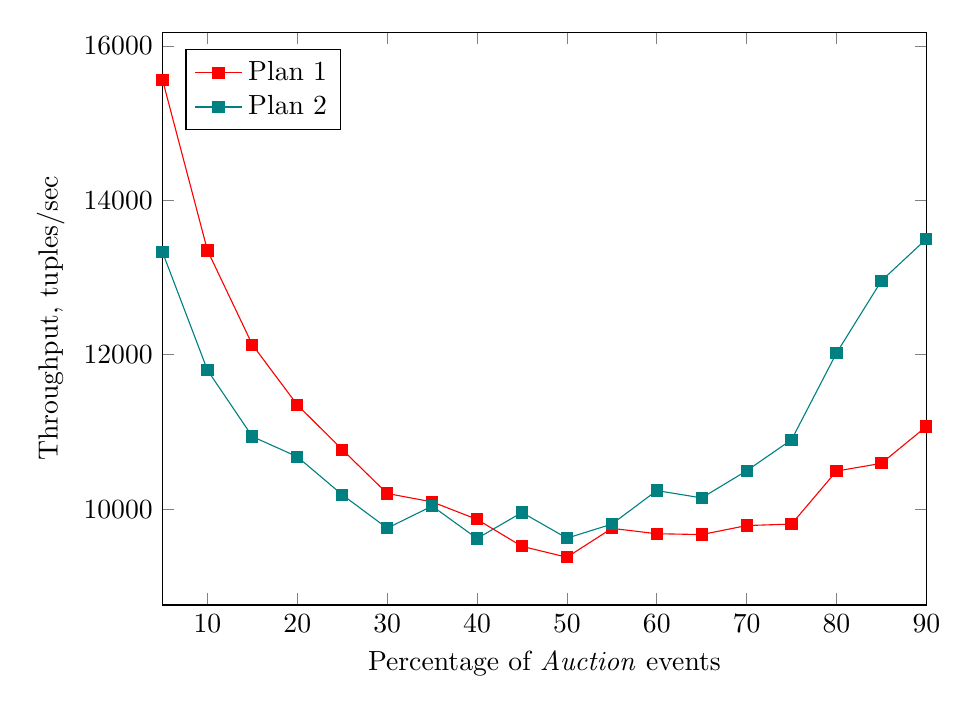
\begin{tikzpicture}
\begin{axis}[
    scale only axis=true,
    width=0.8\textwidth,
    height=0.6\textwidth,
    ytick={10000, 12000, 14000, 16000},
    % yticklabels={3000, 4000, 5000, 6000},
    xmin=5, xmax=90,
    legend cell align=left,
    legend pos=north west,
    xlabel={Percentage of \textit{Auction} events},
    ylabel={Throughput, tuples/sec},
    scaled ticks=false,
     /pgf/number format/.cd,
        use comma,
        1000 sep={}
    % x label style={at={(axis description cs:0.5,0.05)},anchor=north},
    % y label style={at={(axis description cs:0.125,0.5)},anchor=center},
]
\addplot[red,mark=square*,mark options={scale=1,solid}] coordinates {
    (5, 15559.14)
    (10, 13350.6)
    (15, 12128.8)
    (20, 11350.53)
    (25, 10771.7)
    (30, 10203.63)
    (35, 10094.87)
    (40, 9868.2)
    (45, 9519.33)
    (50, 9378.13)
    (55, 9752.17)
    (60, 9682.7)
    (65, 9671.77)
    (70, 9788.26)
    (75, 9807.67)
    (80, 10493.63)
    (85, 10594.13)
    (90, 11070.23)
};
\addplot[teal,mark=square*,mark options={scale=1,solid}] coordinates {
    (5,  13327.4)
    (10, 11800.3)
    (15, 10940.43)
    (20, 10679.2)
    (25, 10187.03)
    (30, 9754.23)
    (35, 10040.93)
    (40, 9621.1)
    (45, 9957.7)
    (50, 9625.23)
    (55, 9806.83)
    (60, 10241.43)
    (65, 10146.33)
    (70, 10497.6)
    (75, 10899.6)
    (80, 12021.9)
    (85, 12957.1)
    (90, 13499.33)
};
\legend{
    Plan 1\\
    Plan 2\\
}
\end{axis}
\end{tikzpicture}